\section[Gewöhnliche DG I]{Gewöhnliche Differentialgleichungen und deren Lösungsansätze}
\Einleitung{Der nächste Themenblock scheint zunächst abgekoppelt von den bisherigen Themen der Vorlesung, allerdings werden wir gerade für die Eindeutigkeitssätze viele der bisher erarbeiteten Begriffe und Sätze (z. B. Lipschitzstetigkeit oder den banachschen Fixpunktsatz) wieder benutzen.\\
Wofür braucht man eigentlich Differentialgleichungen? Als Physikerinnen und Physiker wisst ihr, dass diese ganz natürlich bei der Betrachtung der Trajektorien von massebehafteten Körpern auftreten. Andere Anwendungen finden sich z. B. in der Quantenmechanik (Stichwort: Schrö\-ding\-ergleichung), der Beschreibung von Wärmeausbreitung oder auch in anderen wissenschaftlichen Gebieten wie der Chemie oder Biologie und in der Wirtschaft.\\
Wir hoffen, dass eure Integrierskills nicht eingerostet sind, denn ihr werdet sie brauchen!}

\subsection{Einführung in gewöhnliche Differentialgleichungen}
\subsubsection{Einige Definitionen}
\begin{Def}{Differentialgleichung}
Eine \red{Differentialgleichung} (kurz: DG) ist eine Gleichung, deren Lösung eine Funktion einer oder mehrerer Variablen ist.\\
Eine \red{DG $n$-ter Ordnung} enthält maximal $n$-te Ableitungen der Funktion.
\end{Def}

\begin{Def}
{Gewöhnliche DG}
Die Lösungsfunktionen \red{gewöhnlicher Differentialgleichungen} sind nur von \underline{einer} Variablen (z. B. $x(t)\to$ nur von $t$) abhängig.
\end{Def}
Eine weiter wichtige Klasse von DG, die ihr in Mathe 3 kennenlernt, sind \red{partielle Differentialgleichungen}, bei denen die Lösung von mehreren Variablen abhängt. Es gibt noch weitere Arten, mit denen ihr wahrscheinlich nicht in Kontakt kommen werdet.\\
\blue{Es folgen ein paar genauere Definitionen (analog zum \Skript{}):}
\begin{Def}
{Begriffe zu gewöhnlichen DG erster Ordnung}
Wir betrachten eine Gleichung der Form
\begin{equation*}
    x'(t)=F(x,t).
\end{equation*}
\begin{itemize}
    \item Die Definitionsmenge der Variablen ist $\Omega\subseteq\mathbb{R}\times\mathbb{R}$.\\
    Aus dieser stammen jeweils Paare von $x$ und $t$.
    \item Die Funktion der rechten Seite $f:\Omega\to \mathbb{R}$ hängt dann von $x$ und $t$ ab, wir fordern Stetigkeit.
    \item Die Gleichung $x'=f(x,t)$ nennen wir (explizite) gewöhnliche DG erster Ordnung in $x$.
    \item Eine Lösung auf dem Intervall $I\subseteq\mathbb{R}$ ist eine Funktion $\varphi:I\to\mathbb{R},\,t\mapsto\varphi(t)$, die auf $I$ differenzierbar sein muss.
    \item Die Lösungsfunktion muss die Eigenschaft haben, dass $(\varphi(t),t)\in\Omega\,\forall t\in I$ liegt, und dass $\varphi'(t)=f(\varphi(t),t)\,\forall t\in I$ ist. $\varphi$ muss also die DG lösen, wenn sie in diese eingesetzt wird.
    \item Wir sprechen von einem \red{Anfangswertproblem} (AWP), wenn $\varphi(t_0)=c$ mit $t_0\in I,\,c\in\mathbb{R}$ vorgegeben ist. $\varphi$ ist dann die Lösung der DG mit Anfangsbedingung $x(t_0)=c$.
\end{itemize}
\end{Def}
\begin{Beispiel}
{Veranschaulichung der Definitionen}
Sei $\Omega=\mathbb{R}\times\mathbb{R}$, $f:\Omega\to\mathbb{R},\,f(x,t)=\frac{1}{2}t^3$ stetig mit $x(t_0=1)=4$, so haben wir mit der DG
\begin{equation*}
    x'=f(x,t)=\frac{1}{2}t^3
\end{equation*}
ein Anfangswertproblem.\\
Mit $I=\mathbb{R}$ ist $\varphi:I\to\mathbb{R},\,\varphi(t)=2t^4+c$ eine Lösung.\\
Da $\varphi(1)=4\iff \varphi(t)=2t^4+2$.
\end{Beispiel}
\blue{Dies ist ein einfaches Beispiel, wir werden später sehen, wie man schwierigere Gleichungen löst.}
\begin{Def}
{Begriffe zu gewöhnlichen DG höherer Ordnung}
Wir betrachten eine Gleichung der Form
\begin{equation*}
    x^{(k)}(t)=F(x, x',\ldots,x^{(k-1)},t).
\end{equation*}
\begin{itemize}
    \item Die Definitionsmenge der Variablen ist $\Omega\subseteq\mathbb{R}^k\times\mathbb{R}$.\\
    Aus dieser stammen jeweils die Variablen $(x, x',\ldots,x^{(k)})$ und $t$.
    \item Die Funktion der rechten Seite $f:\Omega\to \mathbb{R}$ hängt dann von $(x, x',\ldots,x^{(k)})$ und $t$ ab, wir fordern Stetigkeit.
    \item Die Gleichung $x^{(k)}=f(x,\ldots, x^{(k-1)},t)$ nennen wir (explizite) gewöhnliche DG $k$-ter Ordnung in $x$.
    \item Eine Lösung auf dem Intervall $I\subseteq\mathbb{R}$ ist eine Funktion $\varphi:I\to\mathbb{R},\,t\mapsto\varphi(t)$, die auf $I$ $k$-fach differenzierbar sein muss.
    \item Die Lösungsfunktion muss die Eigenschaft haben, dass $(\phi(t),t)\in\Omega\,\forall t\in I$ (mit $\phi(t)=(\varphi(t),\ldots,\varphi^{(k-1)})$) liegt, und dass $\varphi^{(k)}(t)=f(\phi(t),t)\,\forall t\in I$ ist. $\varphi$ muss also die DG lösen, wenn sie in diese eingesetzt wird.
    \item Wir sprechen von einem \red{Anfangswertproblem} (AWP), wenn $\varphi(t_0)=c_1,\ldots,\varphi^{(k-1)}(t_0)=c_k$ mit $t_0\in I,\,\cvec\in\mathbb{R}^k$ vorgegeben ist. $\varphi$ ist dann die Lösung der DG mit Anfangsbedingung $\phi(t_0)=\cvec$.
\end{itemize}
\end{Def}
\begin{Beispiel}
{Schwingungsgleichung harmonischer Oszillator}
Die Funktion\footnote{die aus $\mathbb{R}^2\times \mathbb{R}$ abbildet} $f(x,x',t)=-\lambda x$ mit $\lambda \in\mathbb{R}_+$\footnote{entspricht z. B. der Rückstellkonstante $\lambda=\frac{k}{m}$} als DG 2. Ordnung mit $x(t_0=0)=5$\footnote{Entspricht der Auslenkung um 5 Längeneinheiten bei $t=0$}, $x'(0)=15$\footnote{Entspricht der Geschwindigkeit bei $t=0$} können wir in der Differentialgleichung
\begin{equation*}
    x''=-\lambda x
\end{equation*}
betrachten.\\
Hierbei ist eine Lösung $\phi(t)=c_1\sin(\sqrt{\lambda}t+c_2)$.\\
Also ist $\varphi(0)=5=c_1\sin(c_2)$ und $\varphi'(0)=15=c_1\sqrt{\lambda}\cos(c_2)$.\\
Um $c_1$ und $c_2$ zu ermitteln, teilen wir die Gleichungen:\\
$c_2=\arctan(1/(3\sqrt{\lambda})\implies c_1=\frac{5}{\sin(\arctan(1/(3\sqrt{\lambda}))}\overset{\footnote{Vgl. Notizen 9, $\sin(\arctan(b/a))=\frac{b}{\sqrt{a^2+b^2}}$}}{=}5\sqrt{1+9\lambda}$.\\
Somit ist $\varphi(t)=5\sqrt{1+9\lambda}\sin(\sqrt{\lambda}t+\arctan(1/(3\sqrt{\lambda}))$.
\end{Beispiel}

Häufig sind wir an vektoriellen Lösungen interessiert - schon die Beschreibung des Ortes eines Körpers im $\mathbb{R}^3$ führt schnell auf ein System von drei gewöhnlichen DG zweiter Ordnung. Formal ist das so definiert:
\begin{Def}
{Systeme gewöhnlicher Differentialgleichungen}
Wir betrachten eine Gleichung der Form
\begin{equation*}
    \xvec^{(k)}(t)=\Fvec(\xvec, \xvec',\ldots,\xvec^{(k-1)},t).
\end{equation*}
\begin{itemize}
    \item Die Definitionsmenge der Variablen ist $\Omega\subseteq(\mathbb{R}^n)^k\times\mathbb{R}$.\\
    Aus dieser stammen jeweils die Vektoren $(\xvec, \xvec',\ldots,\xvec^{(k)})$ und $t$.
    \item Die Funktion der rechten Seite $f:\Omega\to \mathbb{R}^n$ hängt dann von $(\xvec, \xvec',\ldots,\xvec^{(k)})$ und $t$ ab, wir fordern Stetigkeit.
    \item Die Gleichung $\xvec^{(k)}=\Fvec(\xvec,\ldots, \xvec^{(k-1)},t)$ nennen wir System von gewöhnlichen DG $k $-ter Ordnung in $\xvec$.
    \item Eine Lösung auf dem Intervall $I\subseteq\mathbb{R}$ ist eine Funktion $\varphivec:I\to\mathbb{R}^n,\,t\mapsto\varphivec(t)$, die auf $I$ $k$-fach differenzierbar sein muss.
    \item Die Lösungsfunktion muss die Eigenschaft haben, dass $(\phi(t),t)\in\Omega\,\forall t\in I$ (mit $\phi(t)=(\varphivec(t),\ldots,\varphivec^{(k-1)})$) liegt, und dass $\varphivec^{(k)}(t)=\Fvec(\phi(t),t)\,\forall t\in I$ ist. $\varphivec$ muss also die DG lösen, wenn sie in diese eingesetzt wird.
    \item Wir sprechen von einem \red{Anfangswertproblem} (AWP), wenn $\varphivec(t_0)=\cvec_1,\ldots,\varphivec^{(k-1)}(t_0)=\cvec_k$ mit $t_0\in I,\,\cvec\in(\mathbb{R}^n)^k$ vorgegeben ist. $\varphivec$ ist dann die Lösung der DG mit Anfangsbedingung $\phi(t_0)=\cvec$.
\end{itemize}
\end{Def}

\subsubsection{Reduktion auf DG erster Ordnung}
Wir können höhere $k$-te Ableitungen jeweils als Ableitung der $(k-1)$-ten Ableitung ausdrücken und unser DG-System mit $n$ Gleichungen $k$-ter Ordnung auf ein DG-System mit $k\cdot n$ Gleichungen erster Ordnun reduzieren.\\
Dies rechtfertigt, dass wir vor allem gewöhnliche DG erster Ordnung betrachten.\\
Gerade bei der numerischen Betrachtung von DG spielt dies eine wichtige Rolle.
\begin{Satz}{Satz}
{Reduktion DG höherer Ordnung auf ein System erster Ordnung}
Haben wir so wie oben ein System gewöhnlicher DG vorliegen, so ist äquivalent:
\begin{itemize}
    \item $\xvec:I\to\mathbb{R}^n$ löst ein AWP $k$-ter Ordnung $\xvec^{(k)}=F(\xvec,\ldots,\xvec^{(k-1)}, t)$ und
    \item $\yvec:I\to(\mathbb{R}^n)^k$ löst ein AWP \underline{erster} Ordnung $\yvec'=F^*(\yvec_0,\yvec_1,\ldots,\yvec_{k-1},t)$.
\end{itemize}
Hierbei ist $F^*$ eine Matrix der Dimension $(n\times(k-1))$ und der Vektor $\yvec=(\xvec,\xvec',\ldots)$ enthält die Ableitungen als Komponenten.
\end{Satz}
\begin{Beispiel}
{Erneute Betrachtung der DG 2. Ordnung}
Betrachten wir noch einmal $x''=-\lambda x$.\\
Definieren wir nun den Vektor $\yvec=\MatrixInline{x(t)\\x'(t)}=\MatrixInline{y_0\\y_1}$, so ist
\begin{equation*}
    \yvec'=\MatrixInline{y_0'(t)\\y_1'(t)}=\MatrixInline{x'(t)\\x''(t)}\overset{\footnote{Einsetzen der bestimmenden DG}}{=}\MatrixInline{y_1(t)\\-\lambda y_0(t)}=F^*(y_0,y_1,t).
\end{equation*}
Das ist genau das, was wir wollten - wir haben also ein System mit zwei Gleichungen 1. Ordnung gefunden, zusammengefasst
\begin{equation*}
    \Matrix{y_0'\\y_1'}=\Matrix{0&1\\-\lambda &0}\Matrix{y_0\\y_1}.
\end{equation*}
\blue{Bleibt nur noch die Frage, wie wir sowas lösen können... Dazu mehr unten.}
\end{Beispiel}
\subsubsection{Weitere Definitionen}
\begin{Def}
{Autonome DG}
Hängt die rechte Seite nicht von $t$ ab, so nennen wir die DG \red{autonom}.\\
Sie ist dann von der Form $x^{(k)}=F(x,x',\ldots,x^{(k-1)})$.
\end{Def}
\begin{Def}
{Stetiges Vektorfeld}
Wir nennen eine Abbildung $V$ von $U\subseteq \mathbb{R}^n$ (offen) ein \red{(stetiges) Vektorfeld}, wenn $V:U\to\mathbb{R}^n$ stetig ist.
\end{Def}
\begin{Def}
{Integralkurve}
Eine stetig differenzierbare Abbildung
\begin{equation*}
    \gamma_{x_0}:(-\epsilon,\epsilon)\subseteq\mathbb{R}\to U
\end{equation*}
nennen wir eine \red{Integralkurve} des Vektorfelds $V$ durch $x_0\in U$, wenn $\gamma'(t)=V(\gamma(t))$ mit $\gamma(0)=x_0$ für alle $t\in(-\epsilon,\epsilon)$ ist.\\
\blue{Integralkurven sind also Lösungen einer speziellen autonomen DG mit der Anfangsbedingungn $\gamma(0)=x_0$.}
\end{Def}
\begin{Beispiel}
{Lineares Vektorfeld auf dem $\mathbb{R}^2$ (1/2)}
Für $\lambda\in\mathbb{R}$ definieren wir uns das Vektorfeld $U:\mathbb{R}^2\to\mathbb{R}^2,\,U(x,y)=\lambda\MatrixInline{x\\y}$.\\
Durch den Punkt $\pvec=\MatrixInline{x_0\\y_0}$ ist mit $\gamma_\pvec=e^{\lambda t}\pvec$ eine Integralkurve gegeben, denn
\begin{equation*}
    \gamma'_\pvec(t)=\lambda e^{\lambda t}\pvec=\lambda\gamma_\pvec(t)=U(\gamma_\pvec(t)).
\end{equation*}
\end{Beispiel}
\begin{Beispiel}
{Lineares Vektorfeld mit Veranschaulichung}
Wir betrachten das durch $V(x,y)=\MatrixInline{-y\\x}$ definierte Vektorfeld $V$.\\
Durch die Punkte $\pvec=\MatrixInline{r^2\\0}$ können wir Integralkurven definieren, die dann durch $\gamma_\pvec(t)=r\MatrixInline{\cos(t)\\\sin(t)}$ definiert sind, weil $\gamma'_\pvec(t)=r^2\MatrixInline{-\sin(t)\\\cos(t)}=V(\gamma_\pvec(t))$ ist.\\
\begin{center}
    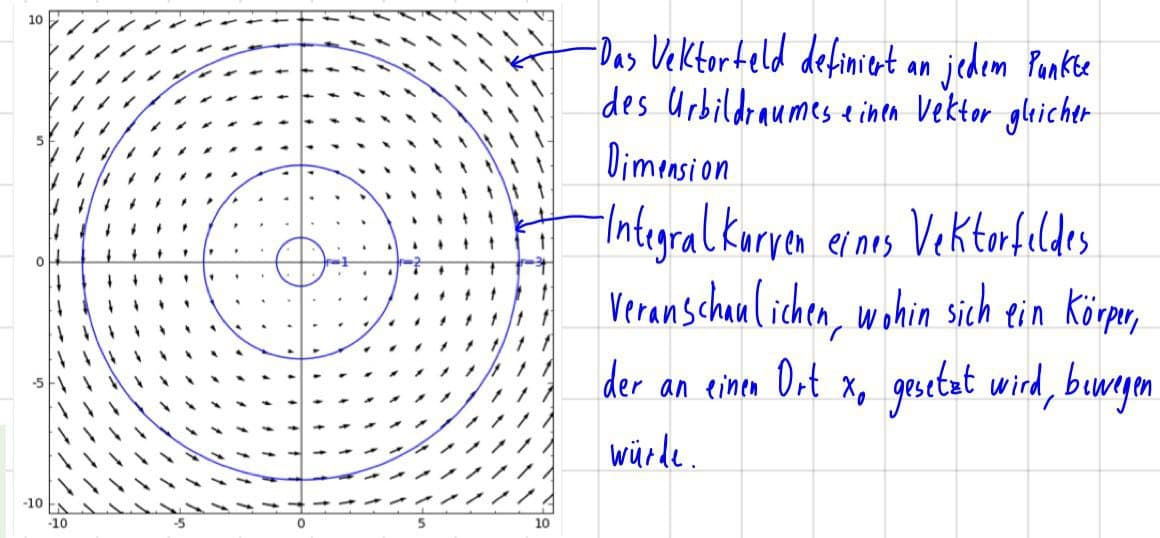
\includegraphics[width=.5\textwidth]{Dateien/11/11Veranschaulichungen.jpg}
\end{center}
\end{Beispiel}


\subsection{Lösungsverfahren}
\blue{Wie löst man aber nun solche DG?\\
Die Ansätze zur Lösung unterscheiden sich von Typ zu Typ, daher ist die Bestimmung des Typs der Differentialgleichung oft schon die halbe Miete.\\
Bei den Lösungsansätzen müsst ihr dann ein paar auswendig lernen\footnote{oder wissen, wo ihr sie nachschlagen könnt...}.}
\subsubsection{Trennung der Variablen}
Eines der einfachsten und am häufigsten verwendeten Lösungsverfahren kann man sich leicht frei nach dem Physikeransatz \textit{wir können ja mal mit dem Differential multiplizieren und dann einfach  integrieren und schauen, ob 'ne Lösung rauskommt} merken.\\
Die Mathematik sagt uns nun, dass das wirklich klappt.\\
\begin{Satz}
{Lösungsansatz}{Trennung der Variablen}
Falls wir die rechte Seite der DG $x'=F(x,t)$ aufteilen können in einen nur von $t$ und einen nur von $x(t)$ abhängigen Anteil eines Produktes, d. h.
\begin{equation*}
    x'(t)=f(t)g(x(t)),
\end{equation*}
was wir als DG mit getrennten Variablen mit Anfangsbedingung $x(t_0)=x_0$ bezeichnen, so ist die Lösung gegeben durch
\begin{equation*}
    x(t)=G^{-1}\BracedInSqr{G(x_0)+\int_{t_0}^tf(s)ds}.
\end{equation*}
Hierbei ist $G(x)$ die Stammfunktion von $\frac{1}{g(x)}$ und $G^{-1}(x)$ deren Umkehrfunktion.\\
\blue{Voraussetzungen sind zudem, dass $f:I_1\to\mathbb{R}$ und $g:I_2\to\mathbb{R}\setminus\MengeDirekt{0}$ stetige Funktionen auf offenen Intervallen $I_1$ und $I_2$ mit $t\in I_1$ und $x\in I_2$ sind.\\
Die Lösung ist dann definiert auf dem Intervall $J\setminus I_1$.}\\
Das Intervall $J$ ist gegeben durch
\begin{equation*}
    \Menge{t\in\mathbb{R}}{G(x_0)+\int_{t_0}^tf(s)ds\in\im(G)}\subseteq I_1\subseteq \mathbb{R}.
\end{equation*}
\end{Satz}
\blue{Bei solchen Sätzen ist es immer wichtig, sowohl die Existenz als auch Eindeutigkeit der Lösung zu zeigen. Wir haben dazu weiter unten noch ein bisschen was geschrieben, ansonsten lohnt sich wie immer der Blick ins \Skript{}.}
\begin{Beispiel}
{Autonome DG sind getrennt (1/3)}
Alle \underline{autonomen} Differentialgleichungen, bei denen die rechte Seite ja nicht von $t$ abhängt, sind DG mit getrennten Variablen.\\
Es ist dann $x=g(x)$ mit $x(t_0)=x_0$ und $x(t)=G^{-1}\BracedInSqr{t+G(x_0)-t_0}$ ist die Lösung, wenn $G$ Stammfunktion zu $\frac{1}{g}$ ist.
\end{Beispiel}
\begin{Beispiel}
{Eine autonome DG (2/3)}
Wir betrachten $\boxed{x'=4x^2+1}$ mit $x(0)=c\in\mathbb{R}$.\\
In diesem Fall ist $g(x)=4x^2+1$ und $f(t)=1$. Also ist
\begin{equation*}
    G(x)=\int \frac{1}{g(x)}dx=\int \frac{1}{1+4x^2}dx=\frac{1}{2}\arctan(x)
\end{equation*}
eine Stammfunktion\footnote{Integrationskonstanten sind hierbei egal, da diese durch die Umkehrfunktion und Einsetzen von $G(x_0)$ aufgehoben werden.} zu $\frac{1}{g}$ mit der Umkehrfunktion $G^{-1}(x)=\tan(2x)$.\\
Die Lösung ist nach obigem Satz also gegeben durch
\begin{equation*}
    x(t)=G^{-1}(t+\frac{1}{2}\arctan(x_0)-t_0)=\tan(2(t+1/2\arctan(c)-0))=\tan(2t+\arctan(c)).
\end{equation*}
Auf welchem Intervall ist diese nun definiert?\\
Das Bild von $G(x)=\frac{1}{2}\arctan(x)$ ist $\BracedIn{-\frac{\pi}{4},\frac{\pi}{4}}$, d. h\\
$J=\Menge{t\in\mathbb{R}}{\frac{1}{2}\arctan(c)+t\in\BracedIn{-\frac{\pi}{4},\frac{\pi}{4}}}$.\\
Formen wir dies um, so finden wir als Intervall $J=(-\frac{\pi}{4}-\frac{1}{2}\arctan(c),\frac{\pi}{4}-\frac{1}{2}\arctan(c))$.\\
\red{Informeller Weg:}\\
\blue{Dieser Lösungsweg ist besser zu merken, ihr könnt ihn z. B. auf Schmierzetteln anwenden und dann zeigen, dass eure gefundene Lösung die DG erfüllt und aufgrund der Eindeutigkeitssätze die einzig mögliche Lösung ist.}\\
\begin{alignat*}{3}
    &&\diff{x}{t}&=1+4x^2\\
    \overset{\cdot dt\tx{\Lightning}}{\iff}&&\int_{x_0}^x\frac{dx}{1+4x^2}&=\int_{t_0}^tdt\\
    \iff&&\frac{1}{2}\arctan(x)-\frac{1}{2}\arctan(x_0)&=t-t_0\\
    \overset{\alpha:=\arctan(x_0)-2t_0}{\iff}&&\arctan(x)&=2t+\alpha\\
    \iff&&x(t)&=\tan(2t+\alpha)\\
    \overset{x(0)=c}{\implies}&&c&=\tan(\alpha)\\
    \iff &&x(t)=\tan(2t+\arctan(c))
\end{alignat*}
\end{Beispiel}
\begin{Beispiel}
{Weitere trennbare gewöhnliche DG (3/3)}
Wir suchen eine Lösung zu $\boxed{x'=\frac{\sin^2(t)}{9x^2}},\,x\neq0$ mit $f(t)=\sin^2(t)$ und $g(x)=\frac{1}{9x^2}$ für $x(0)=\sqrt[3]{c}$, $c\in\mathbb{R}$.\\
Hier ist $G(x)=\int 9x^2dx=3x^3$ eine Stammfunktion zu $\frac{1}{g}$ mit der Umkehrfunktion $G^{-1}(x)=\sqrt[3]{\frac{x}{3}}$.\\
Zudem ist
\begin{equation*}
    \int_0^t\sin^2(s)ds\overset{\footnote{partielle Integration, Umformen der Gleichung}}{=}\BracedInSqr{\frac{1}{2}\BracedIn{s-\sin(s)\cos(s)}}_0^t=\frac{t}{2}-\frac{1}{2}\sin(t)\cos(t).
\end{equation*}
Die Lösung ist also 
\begin{equation*}
    x(t)=G^{-1}\BracedInSqr{3\sqrt[3]{c}^3+\frac{t}{2}-\frac{1}{2}\sin(t)\cos(t)-0}=\sqrt[3]{c+\frac{t}{6}+\frac{1}{6}\sin(t)\cos(t)}.
\end{equation*}
\end{Beispiel}
Der Lösungsansatz mit der Trennung der Variablen bildet häufig den Grundsatz anderer Lösungen.

\subsubsection{Euler-homogene DG}
\begin{Def}
{Euler-homogene DG}
Ist $f:I\to\mathbb{R}$ stetig, so nennen wir $x'=f\BracedIn{\frac{x(t)}{t}}$ mit $(x,t)$ so, dass $\frac{x}{t}\in I$ liegt, eine \red{Euler-homogene DG}
\end{Def}
\begin{Satz}
{Lösungsansatz}{Lösung von Euler-homogenen DG}
Diese Art von DG löst man am besten mit der Substitution $u(t)=\frac{x(t)}{t}$.\\
Die DG für $u$ lautet dann nach der Kettenregel:
\begin{equation*}
    u'=\frac{1}{t}\BracedInSqr{f(u)-u},
\end{equation*}
was wir mithilfe der Trennung der Variablen lösen und durch Resubstitution auf
\begin{equation*}
    x(t)=t u(t)
\end{equation*}
zurückführen können.
\end{Satz}
\begin{Beispiel}
{Zur Euler-homogenen DG}
Wir betrachten $\boxed{x'=\exp\BracedIn{-2\frac{x}{t}}+\frac{x}{t}}$ auf $(0,\infty)$ mit $x(1)=c\in\mathbb{R}$.\\
Die Substitution $u=\frac{x}{t}$ führt uns zur DG
\begin{equation*}
    u'=\frac{1}{t}\BracedIn{e^{-2u}+u-u}=\frac{e^{-2u}}{t},\quad u(1)=\frac{c}{1}=c.
\end{equation*}
Wir führen eine Trennung der Variablen durch:\\
Mit $g(u)=e^{-2u}$ ist $G(u)=\frac{1}{2}e^{2u}$ eine Stammfunktion zu $\frac{1}{g}$ mit der Umkehrfunktion $G^{-1}(u)=\frac{1}{2}\ln(2u)$. Wir sehen wieder, dass $u\in(0,\infty)$ sein muss.\\
Zudem ist mit $f(t)=\frac{1}{t}$ das Integral $\int_1^t\frac{1}{s}ds=\ln(\Abs{t})$, sodass die Lösung der DG für $u$
\begin{equation*}
    u(t)=G^{-1}\BracedInSqr{\frac{1}{2}e^{2c}+\ln(\Abs{t})}=-\frac{1}{2}\ln\BracedIn{e^{2c}+\ln(\Abs{t})}
\end{equation*}
lautet.\\
Die Lösung für $x(t)$ ist daher $x(t)=t\ln\BracedIn{e^{2c}+\ln(\Abs{t})}$.\\
Diese ist definiert auf $J=\Menge{t\in\mathbb{R}}{\frac{1}{2}e^{2c}+\ln(\Abs{t}}\in(0,\infty)$, denn $\im(G)=\im(\frac{1}{2}e^{2\frac{x}{t}}=(0,\infty)$.\\
Wie lautet nun das Intervall für $t$?\\
Wir betrachten die Grenzen:
\begin{align*}
    \frac{1}{2}e^{2c}+\ln(\Abs{t})<\infty&\implies t\leq \infty\\
    \frac{1}{2}e^{2c}+\ln(\Abs{t})>0&\implies t>e^{-\frac{1}{2}e^{2c}}.
\end{align*}
Also muss $t\in I_1=\BracedIn{e^{-\frac{1}{2}e^{2c}},\infty}$ sein.
\end{Beispiel}
\blue{Keine Angst, falls euch das an Beispielen nicht reicht - einige der folgenden Beispiele benötigen diese Technik erneut.}

\subsubsection{Lineare Differentialgleichungen (erster Ordnung)}
\blue{Bisher haben wir immer den Fall betrachtet, dass wir $F(x,t)$ in die Form $f(t)\cdot g(x)$ bringen können.\\
Was passiert aber, wenn noch ein weiterer von $t$ abhängiger Teil im Spiel ist, den wir nicht ausklammern können?\\
Wir betrachten nun den Spezialfall, dass $g(x)=x$ ist.}
\begin{Def}
{Lineare DG}
Als \red{lineare Differentialgleichungen} bezeichnen wir DG der Form
\begin{equation*}
    x'(t)=p(t)x(t)+q(t).
\end{equation*}
Sie ist also linear mit Steigung $p(t)$ von $x$ abhängig, $q(t)$ nennen wir \red{Störfunktion}.\\
$p(t)$ und $q(t)$ sollen hierbei stetige Funktionen sein.
\end{Def}
\begin{Def}
{Homogene und inhomogene lineare DG}
Wir nennen lineare DG
\begin{itemize}
    \item ...\red{homogen}, wenn $q(t)= 0$.
    \item ...\red{inhomogen}, wenn $q(t)\neq 0$.
\end{itemize}
\end{Def}
\blue{Homogene lineare DG können wir entspannt wie gehabt mithilfe der Trennung der Variablen lösen.}
\begin{Satz}
{Lösungsansatz}{Lösung von homogenen linearen DG}
Die Lösung einer homogenen linearen DG $x'=p(t)x$ wird durch
\begin{equation*}
    x(t)=c \exp\BracedIn{\int p(t)dt}
\end{equation*}
bzw. als AWP mit $x(t_0)=x_0$ durch
\begin{equation*}
    x(t)=x_0\exp\BracedIn{\int_{t_0}^tp(s)ds}
\end{equation*}
gegeben. $c$ ist hierbei eine Konstante.
\end{Satz}
Eine inhomogene DG $x'=p(t)x+q(t)$ lösen wir, indem wir zunächst den homogenen Teil $x'=p(t)x$ lösen.\\
Wir bezeichnen die allgemeine Lösung des \underline{homogenen Teils} einer inhomogen DG mit $x_c$.\\
Die spezielle Lösung der inhomogenen DG nennen wir $x_s$.\\
Alle Lösungen der DG sind dann gegeben durch $x(t)=x_c(t)+x_s(t)$.\\
Wollen wir die spezielle Lösung finden, so gibt es verschiedene Ansätze:
\begin{Satz}
{Lösungsansatz}{Variation der Konstanten zur Lösung inhomogener linearer DG}
\begin{enumerate}
    \item Löse zunächst den homogenen Teil wie oben, um
    \begin{equation*}
        x_c(t)=c\exp\BracedIn{\int p(s)ds}
    \end{equation*}
    zu bestimmen.
    \item Nun nehmen wir an, dass die spezielle Lösung die Form
    \begin{equation*}
        x_s(t)=c(t)\exp\BracedIn{\int p(s)ds}
    \end{equation*}
    habe, wobei $c(t)$ nun von der Zeit abhängt. Diesen Ansatz setzen wir in die DG ein, wobei wir durch die Produktregel neue Terme bekommen.
    \item Damit finden wir, dass
    \begin{equation*}
        c(t)=\int q(t)\exp\BracedIn{-\int p(s)ds}dt.
    \end{equation*}
    \item Setzen wir dies in $x_s$ ein, so haben wir schon die spezielle Lösung gefunden!
\end{enumerate}
\end{Satz}

\begin{Beispiel}
{Beispiel aus der Physik}
In der Physik können wir ein radioaktives Isotop $C$ mit Zerfallskonstante $\lambda_C$ mithilfe einer Reaktion erzeugen, indem wir einen Strahl von Teilchen $b$ auf eine Anzahl von Targetkernen $B$ schießen.\\
Sind $N_B$ Targetkerne vorhanden, der Fluss der Teilchen $b$ sei konstant $\phi_b$ und der Wirkungsquerschnitt der Reaktion sei $\sigma$, so entstehen pro Zeiteinheit $r:=\sigma N_b\phi_b$ Isotope des Typs $C$.\\
Andererseits zerfallen pro Zeiteinheit $\lambda_CN_C$ dieser Isotope, sodass die Änderungsrate der Anzahl $N:=N_C$ durch
\begin{equation*}
    \diff{N}{t}=-\lambda_CN+r
\end{equation*}
beschrieben werden kann. Als Anfangsbedingung wählen wir $N(t=0)=0$, sodass wir ein AWP mit der DG $N'=-\lambda_CN+r$ vorliegen haben.\\
\begin{itemize}
    \item Die Lösung des homogenen Teils $N_c'=-\lambda_CN$ ist
    \begin{equation*}
        N(t)=\alpha \exp\BracedIn{\int-\lambda_Cdt}=\alpha\exp(-\lambda_Ct).
    \end{equation*}
    \item Variation der Konstanten liefert:
    \begin{enumerate}
        \item $N_c(t)$ ist gefunden.
        \item Sei nun $N_s(t)=\alpha(t)e^{-\lambda_Ct}$ die spezielle Lösung.
        \item Mit diesem Ansatz ist
        \begin{equation*}
            \alpha(t)=\int r e^{+\lambda_Ct}dt=\frac{r}{\lambda_C}e^{\lambda_Ct}.
        \end{equation*}
        \item Die spezielle Lösung ist dann
        \begin{equation*}
            N_s(t)=\frac{r}{\lambda_C}.
        \end{equation*}
    \end{enumerate}
    \item Insgesamt haben wir als allgemeine Lösung also
    \begin{equation*}
        N(t)=N_c(t)+N_s(t)=\alpha e^{-\lambda t}+\frac{r}{\lambda_C}.
    \end{equation*}
    \item Um das AWP zu lösen, setzen wir $N(0)=0$ ein und finden $0=\alpha e^0+\frac{r}{\lambda_C}\iff \alpha=\frac{r}{\lambda_C}$.\\
    Somit ist
    \begin{equation*}
        N(t)=\frac{r}{\lambda_C}\BracedIn{1-e^{-\lambda_C t}}.
    \end{equation*}
    Physikalisch entspricht dies einer Sättigung bei $\frac{r}{\lambda_C}$ für $t\to \infty$.
\end{itemize}
\end{Beispiel}
\blue{Keine Angst, falls euch das an Beispielen nicht reicht - einige der folgenden Beispiele benötigen diese Technik erneut.}

\begin{Satz}
{Lösungsansatz}{Ansätze für die spezielle Lösung{,} falls $p$ konstant ist}
Je nachdem, wie die Störfunktion aufgebaut ist, lohnen sich auch wagemutigere Ansätze.\\
Wir betrachten eine DG $x'(t)=px(t)+q(t)$, für die $p\neq0$ konstant sei.
\begin{enumerate}
    \item Ist $q(t)$ ein Polynom $h(t)$ vom Grad $m$ mit reellen Koeffizienten:\\
    Setze ein Polynom $Q$ von Grad $m$ für $x_s(t)$ an, also $x_s(t)=Q(t)=\sum_{k=0}^ma_kt^k$.
    \item Ist $q(t)$ auf die Form $h(t)e^{at}$ zurückzuführen:\\
    Setze $x_s(t)=Q(t)e^{at}$ an, falls $a\neq p$.\\
    Setze $x_s(t)=tQ(t)e^{at}$ an, falls $a=p$.
    \item Ist $q(t)$ auf die Form $h(t)\cos(bt)$ oder $h(t)\sin(bt)$ zurückzuführen:\\
    Setze $x_s(t)=Q_1(t)\cos(bt)+Q_2(t)\sin(bt)$ an.
    \item Ist $q(t)$ auf die Form $h(t)\cos(bt)e^{at}$ oder $h(t)\sin(bt)e^{at}$ zurückzuführen:\\
    Setze $x_s(t)=Q_1(t)e^{at}\cos(bt)+Q_2e^{at}\sin(bt)$ an.
\end{enumerate}
Die Ansätze werden dann in die DG eingesetzt, die Koeffizienten der Polynome $Q_i(t)$ müssen durch Koeffizientenvergleich bestimmt werden.
\end{Satz}
\begin{Beispiel}
{Ansatz für die spezielle Lösung}
Betrachte $x'=\lambda x+(t^2+2t)e^{at}$, wobei $\lambda\in\mathbb{R}\setminus\MengeDirekt{0}$ und $a\in\mathbb{R}, a\neq\lambda$ seien.\\
Dies entspricht dem zweiten Fall, der Grad des Polynoms $h(t)=t^2+2t$ ist $m=2$.\\
Wir wählen also den Ansatz
\begin{equation*}
    x_s(t)=\alpha_0+\alpha_1t+\alpha_2t^2)e^{at}.
\end{equation*}
Setzen wir dies in die DG ein, so ergibt sich
\begin{equation*}
    (\alpha_0+\alpha_1t+\alpha_2t^2+\alpha_1+2\alpha_2t)e^{at}=\lambda \alpha_0+\alpha_1t+\alpha_2t^2)e^{at}+e^{at}(t^2+2t).
\end{equation*}
Der Koeffizientenvergleich liefert nach Division durch $e^{at}$:
\begin{alignat*}{3}
t^0:&&\alpha_0+\alpha_1&=\lambda \alpha_0\\
t^1:&&\alpha_1+2\alpha_2&=\lambda \alpha_1+2\\
t^2:&&\alpha_2&=\lambda\alpha_2+1\iff \alpha_2=\frac{1}{1-\lambda}.
\end{alignat*}
Durch Einsetzen von $\alpha_2$ in die zweite Gleichung folgt
\begin{equation*}
    \alpha_1=\frac{1-2\alpha_2}{1-\lambda}=\frac{2-2/(1-\lambda)}{1-\lambda}=\frac{2-2\lambda-2}{(1-\lambda)^2}=\frac{2\lambda}{(1-\lambda)^2}.
\end{equation*}
Dies können wir in die erste Gleichung einsetzen, um $\alpha_0=-\frac{\alpha_1}{1-\lambda}=-\frac{2\lambda}{(1-\lambda)^3}$ zu erhalten.\\
Die allgemeine Lösung (inklusive der homogenen $x_s(t)=ce^{\lambda t}$) ist dann
\begin{equation*}
    x(t)=ce^{\lambda t}+e^{at}\BracedInSqr{\frac{-2\lambda}{(1-\lambda)^3}+\frac{2\lambda}{(1-\lambda)^2}t+\frac{1}{1-\lambda}t^2}.
\end{equation*}
\end{Beispiel}

\subsubsection{Bernoullische DG}
\begin{Def}
{Bernoullische DG}
Hat die Störfunktion einer linearen DG einen Zusatz $x^\alpha$, sodass die DG die Form
\begin{equation*}
    x'(t)=p(t)x(t)+q(t)x^\alpha(t)
\end{equation*}
hat, wobei $\alpha\in\mathbb{R}\setminus\MengeDirekt{0,1}$ und $p,q:I\to\mathbb{R}$ stetig seien, so bezeichnen wir dies als \red{Bernoullische Differentialgleichung}
\end{Def}
Als Ansatz zur Lösung einer solchen DG substituieren wir geschickt:
\begin{Satz}
{Lösungsansatz}{Bernoullische DG}
Haben wir eine Bernoullische DG der obigen Form vorliegen, so wählen wir $u(t)=\BracedInSqr{x(t)}^{1-\alpha}$.\\
Die neue DG lautet nach Einsetzen
\begin{equation*}
    u'=(1-\alpha)p(t)u+(1-\alpha)q(t),
\end{equation*}
was wieder einer inhomogenen linearen Differentialgleichung entspricht.\\
Durch Resubstitution finden wir als Lösung
\begin{equation*}
    x(t)=\BracedInSqr{u(t)}^\frac{1}{1-\alpha}.
\end{equation*}
\end{Satz}
\begin{Beispiel}
{Bernoullische DG}
Wir betrachten $\boxed{x'=\frac{1}{t}x+\frac{1}{\sqrt{x}}}$.\\
In diesem Fall ist $p(t)=\frac{1}{t}$, $q(t)=1$ und $\alpha=-\frac{1}{2}$.\\
Wir substituieren:
\begin{equation*}
    u(t)=x^{1-\alpha}=x^\frac{3}{2}\implies u'=\underbrace{\BracedIn{1+\frac{1}{2}}\frac{1}{t}}_{=:p_1(t)}u+\underbrace{\BracedIn{1+\frac{1}{2}}}_{=:q_1(t)}.
\end{equation*}
Die homogene Lösung ist dann
\begin{equation*}
    u_c(t)=c\exp\BracedIn{\int p_1(s)ds}=c\exp\BracedIn{\frac{3}{2}\ln(t)}=ct^\frac{3}{2}.
\end{equation*}
Die spezielle Lösung finden wir durch Variation der Konstanten. Wir wählen $u_s(t)=c(t)t^\frac{3}{2}$.\\
Die 'Konstante' ist dann
\begin{equation*}
    c(t)=\int q_1(s)s^{-\frac{3}{2}}ds=\int \frac{3}{2}s^{-\frac{3}{2}}ds=-3t^{-\frac{1}{2}}\implies u_s(t)=-3t^{-\frac{1}{2}}t^\frac{3}{2}=-3t
\end{equation*}
Also ist die allgemeine Lösung für $u$
\begin{equation*}
    u(t)=u_c(t)+u_s(t)=ct^\frac{3}{2}-3t=t\BracedIn{c\sqrt{t}-3}.
\end{equation*}
Resubstitution liefert als Lösung für $x$ dann
\begin{equation*}
    x(t)=\BracedInSqr{u(t)}^\frac{1}{1-\alpha}=\BracedInSqr{t\BracedIn{c\sqrt{t}-3}}^\frac{2}{3}.
\end{equation*}
\end{Beispiel}


\subsubsection{Exakte DG}
Mit der folgenden Art von Differentialgleichungen schlagt ihr euch in der Thermodynamik viel rum.
\begin{Def}
{Exakte DG}
Wir betrachten die stetig differenzierbaren Funktionen $P,Q:U\to\mathbb{R}$, wobei $U\subseteq\mathbb{R}^2$ offen und wegzusammenhängend sei.\\
Für diese Funktion soll auf $U$ die sog. \red{Integrabilitätsbedingung} gelten: 
\begin{equation*}
    \diffp{P}{x}=\diffp{Q}{t},\quad Q\neq0.
\end{equation*}
Eine DG der Form $P(t,x(t))+Q(t,x(t))x'(t)=0$ nennen wir \red{exakte Differentialgleichung}. 
\end{Def}
\begin{Satz}
{Lösungsansatz}{Methode zum Lösen exakter DG}
Als Lösungsansatz für eine DG mit Anfangsbedingung $x(t_0)=x_0$ suchen wir eine $C^2$-Potentialfunktion\footnote{also eine zweimal stetig differenzierbare Funktion} $F(x,t)$ mit $\diffp{F}{t}=P$ und $\diffp{F}{x}=Q$.\\
Die DG können wir dann durch Auflösen der Gleichung $F(x,t)=F(x_0,t_0)$ nach $x$ lösen.
\end{Satz}
\begin{Satz}
{Lösungsansatz}{Exakte DG ohne Integrabilitätsbedingung}
Ist die Integrabilitätsbedingung $\diffp{P}{x}=\diffp{Q}{x}$ für die Gleichung $P(t,x(t))+Q(t,x(t))x'(t)=0$ \underline{nicht} erfüllt,\\
so kann ein integrierender Faktor $\lambda(x,t)\neq0$ mit $\diffp{\lambda P}{x}=\diffp{\lambda Q}{t}$ die DG in die exakte Form
\begin{equation*}
    \lambda P+ \lambda Q x'=0
\end{equation*}
bringen.
\end{Satz}

\begin{Beispiel}
{Eine nicht exakte DG}
Wir betrachten die DG $\boxed{-5t+4x+2tx'=0}$.\\
In diesem Fall ist $P(x,t)=-5t+4x$, $Q(x,t)=2t$.\\
Weil $\diffp{P}{x}=4\neq2=\diffp{Q}{t}$ ist die DG nicht exakt!\\
Durch Überlegen kommen wir auf den integrierenden Faktor $\lambda(x,t)=t$.\\
In diesem Fall ist $\lambda P+\lambda Qx'=0\implies -5t^2+4tx+2t^2x'=0$.\\
Weil jetzt $\diffp{\lambda P}{x}=4t=\diffp{\lambda Q}{t}$, liegt nun eine exakte DG vor!\\
Wir suchen als nur eine Funktion $F(x,t)$ mit $\diffp{F}{t}=\lambda P$ und $\diffp{F}{x}=\lambda Q$.\\
Dafür integrieren wir beide Seiten:
\begin{align*}
    F&=\int \lambda Q dx=\int 2t^2dx=2t^2x+c(t)\\
    F&=\int \lambda P dt=\int(-5t^2+4tx)dt=-\frac{5}{3}t^3+2t^2x+c(x).
\end{align*}
Achtung, bei der Integration hängen die Konstanten jeweils noch von der anderen Variablen ab!\\
Wir sehen also, dass die kombinierte Funktion $F(x,t)=2t^2x-\frac{5}{3}t^3$ eine Potentialfunktion ist.\\
Die Anfangsbedingung sei $x(t_0)=x_0$.\\
Dann muss $F(x,t)=F(x_0,t_0)$ sein:
\begin{equation*}
    \iff 2t^2x-\frac{5}{3}t^3=2t_0^2x_0-\frac{5}{3}t_0^3\implies x(t)\frac{1}{2t^2}\BracedInSqr{2t_0^2x_0+\frac{5}{3}(t^3-t_0^3)}
\end{equation*}
\end{Beispiel}
Im \Skript{} findet ihr weitere Beispiele zu exakten DG!

\subsubsection{Abschlussbeispiele}
Zum Abschluss betrachten wir noch einmal zwei schöne Beispiele:
\begin{Beispiel}
{Anfangswertproblem mit exotischer Substitution (1/2)}
Wir betrachten $\boxed{x(1+t)x'=x^2-1-(1-t)^2}$ für $t>0$ mit $x(0)=1$.\\
Wir wählen die Substitution $u(t)=1-x^2(t)$ (versucht es mit diesem Ansatz gerne selbst!).\\
Dann ist nach der Kettenregel
\begin{equation*}
    u'(t)=-2x(t)x'(t) =-2\frac{x^2-1-(1+t)^2}{1+t}=2(1+t)+2\frac{u}{1+t},
\end{equation*}
wobei wir $x'$ aus der DG eingesetzt und $u$ wieder identifiziert haben.\\
Typanalyse: Dies ist eine lineare DG mit $p(t)=\frac{2}{1+t}$ und $q(t)=2+2t$.
\begin{itemize}
    \item \textbf{Homogene Lösung}:
    \begin{equation*}
        u_c(t)=c\exp\BracedIn{\int p(s)ds}=c\exp(2\ln(\Abs{1+t})\overset{t>0}{=}c(1+t)^2.
    \end{equation*}
    \item \textbf{Spezielle Lösung}:\\
    Sei $u_s(t)=c(t)(1+t)^2$.
    \begin{equation*}
        c(t)=\int q(s)\exp\BracedIn{-\int p(y)dy}ds=\int 2(1+s)(1+s)^{-2}ds\overset{t>0}{=}2\ln(1+t).
    \end{equation*}
    \item \textbf{Allgemeine Lösung}:\\
    Wir haben also
    \begin{equation*}
        u(t)=u_c(t)+u_s(t)=c(1+t)^2+2\ln(1+t)(1+t)^2.
    \end{equation*}
\end{itemize}
Eine Resubstitution liefert uns
\begin{equation*}
    x(t)=\pm\sqrt{1-u(t)}=\pm \sqrt{1-(1+t)^2(c+2\ln(1+t))}.
\end{equation*}
Die Anfangsbedingung $x(0)=1$ führt uns nun auf $1\overset{!}{=}\pm\sqrt{1-1}2(c+\ln(1))\iff c=0$, wir müssen die positive Lösung wählen. Also ist
\begin{equation*}
    x(t)=\sqrt{1-2(1-t)^2\ln(1+t)}.
\end{equation*}
\end{Beispiel}

\begin{Beispiel}
{Separation der Variablen reloaded (2/2)}
Wir betrachten das AWP $\boxed{t^2xx'=e^{x^2}}$ für $t>0$ mit $x(1)=0$.\\
Separation der Variablen führt uns zur Darstellung
\begin{equation*}
    x'=\frac{e^{x^2}}{x}\frac{1}{t^2}=:g(x)f(t).
\end{equation*}
Hier ist die Stammfunktion $G$ zu $\frac{1}{g}$ gegeben durch
\begin{equation*}
    G(x)=\int s e^{-s^2}ds\overset{\tx{Subst. }z=s^2}{=}\int\frac{1}{2}e^{-z}dz=\frac{-1}{2}e^{-x^2}
\end{equation*}
mit der Umkehrfunktion $G^{-1}(x)=\pm\sqrt{-\ln(-2x)}$.\\
Zudem ist
\begin{equation}
    \int_{t_0}^tf(s)ds=\int_1^t\frac{1}{s^2}ds=-\frac{1}{t}+1.
\end{equation}
Gemäß des Satzes über die Trennung der Variablen ist die Lösung somit
\begin{align*}
    x(t)&=G^{-1}\BracedInSqr{G(x_0)+\int_{t_0}^tf(s)ds}=G^{-1}\BracedInSqr{-\frac{e^0}{2}-\frac{1}{t}+1}\\
    &=\pm\sqrt{-\ln\BracedInSqr{-2\BracedIn{\frac{1}{2}-\frac{1}{t}}}}=\pm\sqrt{-\ln\BracedIn{\frac{2}{t}-1}}=\pm\sqrt{\ln\BracedIn{\frac{t}{2-t}}}.
\end{align*}
Da $\ln(x)$ nur für $x>0$ definiert ist, muss $\frac{t}{2-t}>0\iff t<2$ sein.\\
Zudem ist $\ln(x)$ negativ für $x<1$, die Wurzel aber nicht für negative Zahlen definiert. Somit muss $\frac{t}{2-t}\geq1\iff t\geq1$ sein.\\
Die Lösung des AWP sind also die Funktionen
\begin{equation*}
    x(t)=\pm\sqrt{\ln\BracedIn{\frac{t}{2-t}}},\quad t\in[1,2).
\end{equation*}
\end{Beispiel}